\documentclass{article}

\usepackage{amsmath}
\usepackage{multicol}
\usepackage{titlesec}
\usepackage{enumitem}
\usepackage{adjustbox}
\usepackage{stmaryrd}
\usepackage{tikz}
\setlist{nosep}
\titleformat{\subsection}[runin]{\normalfont\Large\bfseries}{\thesubsection.}{6pt}{}[]
\titlespacing*{\subsection}{0pt}{0pt}{0pt}



% Disable warnings
% chktex-file 1

\usepackage[margin=0.45in, portrait]{geometry} % may exceed print margins
\pagestyle{empty}

\usepackage[dvipsnames]{xcolor}

% Colour-blind friendly scheme
\definecolor{MyMagenta}{rgb}{0.91,0.16,0.54}
\definecolor{MyGreen}{rgb}{0.4,0.65,0.12}
\definecolor{MyPurple}{rgb}{0.46,0.44,0.7}
\definecolor{MyOrange}{rgb}{0.85,0.37,0.01}
\definecolor{MyEmerald}{rgb}{0.11,0.62,0.47}
\definecolor{MyYellow}{RGB}{230,171,2}
\definecolor{MyBlue}{RGB}{0,114,178}

\colorlet{defc}{MyMagenta}
\colorlet{lemc}{MyGreen}
\colorlet{corc}{MyPurple}
\colorlet{propc}{MyOrange}
\colorlet{thmc}{MyEmerald}
\colorlet{alg}{MyYellow}
\colorlet{ex}{MyBlue}

\colorlet{namec}{DarkOrchid}

\newcommand{\wde}[1]{\textcolor{defc}{\newline\textbf{DEF}} (\textcolor{namec}{\textit{#1}})}
\newcommand{\wl}[1]{\textcolor{lemc}{\newline\textbf{LEM}} (\textcolor{namec}{\textit{#1}})}
\newcommand{\wc}[1]{\textcolor{corc}{\newline\textbf{COR}} (\textcolor{namec}{\textit{#1}})}
\newcommand{\wpr}[1]{\textcolor{propc}{\newline\textbf{PROP}} (\textcolor{namec}{\textit{#1}})}
\newcommand{\wt}[1]{\textcolor{thmc}{\newline\textbf{THM}} (\textcolor{namec}{\textit{#1}})}
\newcommand{\wa}[1]{\textcolor{alg}{\newline\textbf{ALG}} (\textcolor{namec}{\textit{#1}})}
\newcommand{\wpf}[1]{\textcolor{red}{\newline\textit{#1}}}  % Proof
\newcommand{\we}[1]{\textcolor{ex}{\newline\textbf{EX}} (\textcolor{namec}{\textit{#1}})}

\usepackage{amsmath}
\usepackage{amsthm}
\usepackage{amssymb}
\usepackage{tipa}
\usepackage{algpseudocode}
\usepackage{amssymb}
\usepackage{ebproof}

\newcommand{\transp}[1]{#1^\top}
\newcommand{\dotp}[2]{\transp{#1}#2}
\newcommand{\norm}[1]{\left\lVert#1\right\rVert_2} % L_2 norm
\newcommand{\inner}[2]{\left\langle#1,#2\right\rangle} % Inner product
\newcommand{\vect}[1]{\boldsymbol{#1}}

% frobenius norm
\newcommand{\frobnorm}[1]{\left\lVert#1\right\rVert_F}

\newcommand{\pderivative}[2]{\frac{\partial #1}{\partial #2}}


% expectation 
\newcommand{\E}{\mathbb{E}}

% \fontsize{2}

\begin{document}
  \begin{multicols}{2}
  \subsection*{Analytic Geometry}
  \wde{Dot Product}{The dot product between two vectors $u$ and $v$ is defined as 
$$
\dotp{u}{v} = u_1v_1 + u_2v_2 + \ldots + u_nv_n = \sum_{i=1}^n u_iv_i
$$}
\wde{Bilinearity}{
    The dot product is bilinear, i.e. for any vectors $u,v,w$ and scalar $a$,
    \begin{align*}
        \dotp{au}{v} &= a\dotp{u}{v} = \dotp{u}{av} \\
        \dotp{u+v}{w} &= \dotp{u}{w} + \dotp{v}{w} \\
        \dotp{w}{u+v} &= \dotp{w}{u} + \dotp{w}{v}
    \end{align*}
}
\wde{Commutativity}{The dot product is commutative, i.e. $\dotp{u}{v} = \dotp{v}{u}$}
\wde{Inner Product}{
    The inner product between two vectors $u$ and $v$ is defined as 
    $$
    \inner{u}{v}
    $$
    Dot product is a special case of inner product.
}
\wde{$\ell_2$ Norm}{
    The $\ell_2$ norm of a vector $v$ is defined as
    $$
    \norm{v} = \sqrt{\dotp{v}{v}} = \sqrt{v_1^2 + v_2^2 + \ldots + v_n^2}
    $$
    Also called the Euclidean norm.
}

\wde{$\ell_2$ properties}
{
 For all vectors $u,v$ and scalar $a$,
 \begin{itemize}
    \item The $\ell_2$ norm is non-negative, i.e. $\norm{v} \geq 0$.
    \item $\norm{au} = |a|\norm{u}$ for any scalar $a$.
    \item $\norm{u}$ is zero if and only if $u$ is the zero vector.
    \item The triangle inequality holds, i.e. $\norm{u+v} \leq \norm{u} + \norm{v}$.
    \item $\norm{x-y} = \norm{y-x}$, also called symmetry.
    \item $\norm{u+v}^2 = \norm{u}^2 + 2\dotp{u}{v} + \norm{v}^2$
    \item $\cos \theta = \frac{\dotp{u}{v}}{\norm{u}\norm{v}}$ (can be proved using the law of cosines)
 \end{itemize}
}
\wt{Cauchy-Schwarz Inequality}{
    For any vectors $u,v$, the following inequality holds:
    $$
    |\inner{u}{v}| \leq \norm{u}\norm{v}
    $$
}
\wde{Line}{
    A line is a set of points $$\{x : x = u + tv \text{ for some } t \in \mathbb{R}\}$$ where $u$ is a point on the line and $v \neq 0$ is the direction vector.
}
\wde{Plane}{
    A plane is a set of points $$\{ x : \dotp{v}{x-u} = 0 \}$$ where $v$ is the normal vector to the plane and $u$ is the shift from the origin.
}

\wde{Angle between two vectors}{
    The angle $\theta$ between two vectors $u$ and $v$ is given by
    $$
    \cos \theta = \frac{\dotp{u}{v}}{\norm{u}\norm{v}}
    $$
}

\wde{Projection}{
    The vector $\norm{u}\cos \theta \frac{v}{\norm{v}}$ is a projection of $u$ onto $v$. 
    % let's use tikz to draw this 
    % \begin{center}
    %     \begin{tikzpicture}
    %         \draw[->] (0,0) -- (2,0) node[right] {$v$};
    %         \draw[->] (0,0) -- (1,1) node[above] {$u$};
    %         \draw (0.5,0) arc (0:45:0.5);
    %         \node at (0.7,0.2) {$\theta$};
    %         \draw[dashed] (1,1) -- (1,0);
    %     \end{tikzpicture}
    % \end{center}
}
\wde{Distance between a point and a plane}{
    The distance between a point $z$ and a plane $\dotp{v}{x-u} = 0$ is given by
    $$
    \frac{|\dotp{v}{z-u}|}{\norm{v}}
    $$ 
    % TODO draw a diagram
}
\wde{Distance between a point and a line}{
    The distance between a point $z$ and a line $x = u + tv$ is given by
    $$
    \norm{z-u-\frac{\dotp{z-u}{v}}{\norm{v}^2}v}
    $$
    % TODO draw a diagram
}

\wde{Singular Value Decomposition (SVD)}{
    The SVD of a matrix $X$ is $U\Sigma V^T$, where $\dotp{U}{U} = I, \dotp{V}{V} = I$ and $\Sigma$ is a diagonal matrix:
    $$
    \Sigma = \begin{bmatrix}
        \sigma_1 & 0 & \ldots & 0 \\
        0 & \sigma_2 & \ldots & 0 \\
        \vdots & \vdots & \ddots & \vdots \\
        0 & 0 & \ldots & \sigma_n
    \end{bmatrix}
    $$
    and $\sigma_1 \geq \sigma_2 \geq \ldots \geq \sigma_n \geq 0$.
}

\wt{Eckart-Young Theorem}{
    Let $\Sigma_k = \operatorname{diag}(\sigma_1, \ldots, \sigma_k, 0, \ldots, 0)$ where $k \leq d$.
    The matrix $U\Sigma_kV^T$ is the optimal solution to the following problem:
    $$
    \min_{\hat X} \frobnorm{X - \hat X} \text{ s.t. } \operatorname{rank}(\hat X) \leq k
    $$
    The matrices $Z = U\Sigma_k$ and $W = V^T$ are the optimal solution to 
    $$
    \min_{Z,W} \frobnorm{X - ZW} \text{ s.t. } Z \in \mathbb{R}^{n \times k}, W \in \mathbb{R}^{k \times d}
    $$
}
\wt{Useful Identities}{
    \begin{itemize}
        \item $A(\dotp{A}{A})^{-1} = (AA^T)^{-1}A^T$
    \end{itemize}
}

  \subsection*{Calculus}
  \wde{Derivative}{
    The derivative of a function $f : \mathbb{R} \to \mathbb{R}$ at $x_0$ is defined as:
    $$
    (D_x f)(x_0) = \left(\frac{d}{dx} f\right)(x_0) = \lim_{h\to 0} \frac{f(x_0+h) - f(x_0)}{h}
    $$
}
\wde{Directional Derivative}{
    The directional derivative of a function $f : \mathbb{R}^d \to \mathbb{R}$ along 
    the direction $v$ at $x_0 \in \mathbb{R}^d$ is defined as:
    $$
        (D_v f)(x_0) = \lim_{h\to 0} \frac{f(x_0 + hv) - f(x_0)}{h}
    $$
}
\wde{Partial Derivative}{
    The partial derivative is a directional derivative along the 
    direction of coordinate axes. For a function $f : \mathbb{R}^d \to \mathbb{R}$,
    the partial derivative with respect to the $i$-th coordinate is denoted as:
    $$
    \pderivative{f}{x_i} = \lim_{h\to 0} \frac{f(x_1, \ldots, x_i + h, \ldots, x_d) - f(x_1, \ldots, x_i, \ldots, x_d)}{h}
    $$
}
\wde{Gradient}{
    The gradient of a function is the vector consisting of all partial derivatives
    denoted by $\nabla f$ or $\pderivative{f}{x}$. For a function $f : \mathbb{R}^d \to \mathbb{R}$,
}
% reset italics
\we{Gradient Identities}{
    \begin{itemize}
        \item \normalfont Given a function $f(a) = \dotp{b}{a}$, $(\nabla f)(a) = b$ 
        \item Given a function $f(a) = \norm{a}^2$, $(\nabla f)(a) = 2a$
        \item Given a function $f(a) = \dotp{a}{Aa}$, $(\nabla f)(a) = (A + A^T)a$
    \end{itemize}
}
\wde{Hessian}{
    The Hessian of a function $f : \mathbb{R}^d \to \mathbb{R}$ is the matrix of second partial derivatives:
    $$
    \nabla^2 f = \begin{bmatrix}
        \pderivative{^2 f}{x_1^2} & \pderivative{^2 f}{x_1x_2} & \ldots & \pderivative{^2 f}{x_1x_d} \\
        \pderivative{^2 f}{x_2x_1} & \pderivative{^2 f}{x_2^2} & \ldots & \pderivative{^2 f}{x_2x_d} \\
        \vdots & \vdots & \ddots & \vdots \\
        \pderivative{^2 f}{x_dx_1} & \pderivative{^2 f}{x_dx_2} & \ldots & \pderivative{^2 f}{x_d^2}
    \end{bmatrix}
    $$
}
\we{Hessian Example}{
    Given a function $f(x,y) = x^2 - y^2$, the Hessian is:x:
    $$
    \nabla^2 f = \begin{bmatrix}
        2 & 0 \\
        0 & -2
    \end{bmatrix}
    $$
    The 2 indicates that it looks like a cup along the $x$-axis and the -2 indicates that it looks like an upside-down cup along the $y$-axis.
}

  \subsection*{Optimisation}
  \wde{Minimum}{
    The minimum of a function $f : \mathbb{R}^d \to \mathbb{R}$ is written as $\min_{x} f(x)$, and has 
    the property that $\min_{x} f(x) \leq f(y)$ for all $y \in \mathbb{R}^d$.
    The value $x^*$ such that $f(x^*) = \min_{x} f(x)$ is called the minimizer.
}
\wde{Convexity}{
    A function $f : \mathbb{R}^d \to \mathbb{R}$ is convex if for any $0 \leq \alpha \leq 1$, we have
    $$
    f(\alpha x + (1-\alpha)y) \leq \alpha f(x) + (1-\alpha)f(y)
    $$
    In general,
    $$
    f(\sum_{i=1}^k \alpha_i x_i) \leq \sum_{i=1}^k \alpha_i f(x_i)
    $$
}
\wde{Concavity}{
    A function $f$ is concave if $-f$ is convex.
}

\wt{First Order Condition (Convexity)}{
    If $f$ is convex then,
    \begin{itemize}
        \item $f(x) \geq f(y) + \nabla f(y)^\top(x-y)$ 
    \end{itemize}
}

\wde{Positive Semidefinite}{
    A matrix $A$ is positive semidefinite if for all vectors $v \neq 0$ we have $v^\top Av \geq 0$.
    Also written as $A \succeq 0$.
}

\wt{Convex Function Implies Positive Semidefinite Hessian}{
    If $f$ is convex, then $\nabla^2 f(x) \succeq 0$.
}

\wde{Positive Definite}{
    A matrix $A$ is positive definite if for all vectors $v \neq 0$ we have $v^\top Av > 0$.
    Also written as $A \succ 0$.
}

\wde{Affine}{
    A function $f$ is affine if $f(x) = Ax + b$ for some matrix $A$ and vector $b$.
}

\wt{Affine Transform Preservation}{
    If $f$ is convex, then $g(x) = f(Ax + b)$ is also convex.
    % TODO: show proof
}

\wt{Non-negative Weighted Sum}{
    If $f_1, f_2, \ldots, f_k$ are convex functions, then $f(x) = \sum_{i=1}^k \beta_i f_i(x)$ is convex for all $\beta_i \geq 0$.
}

\we{Gradient of Quadratic Form}{
    $\nabla_x (\dotp{x}{Ax}) = (A + A^\top)x$ % called 
}

\wde{Strictly Convex}{
    A function $f : \mathbb{R}^d \to \mathbb{R}$ is called strictly if for $0 \leq \alpha \leq y$ we have
    $$
    f(\alpha x + (1-\alpha)y) < \alpha f(x) + (1-\alpha)f(y)
    $$
    for any $x \neq y$.
}

\wde{First Order Condition (Strict Convexity)}{
    If $f$ is strictly convex then,
    \begin{itemize}
        \item $f(x) > f(y) + \nabla f(y)^\top(x-y)$ 
    \end{itemize}
}
\wt{Unique Minimizer}{
    If $f$ is strictly convex, then $f$ has a unique minimizer.
}

\wt{Jensen's Inequality}{
    If a function $f$ is convex,
    $$
    f(\E_{x \sim p}[x]) \leq \E_{x \sim p}[f(x)]
    $$
}

\wde{Gradient Descent}{
    The gradient descent algorithm is given by
    $$
    x_{t+1} = x_t - \eta \nabla f(x_t)
    $$
    where $\eta$ is the learning rate/step size.
}

% sublinear, linear and quadratic convergence
\wde{Convergence}{
    Given $\epsilon > 0$, we say that an algorithm converges to a point $x^*$ if 
    $$
    f(x_t) - f(x^*) \leq \epsilon 
    $$
}

\wde{Convergence Rate}{
    The convergence rate of an algorithm is the rate at which the algorithm converges to the optimal point.
    There are three types of convergence rates:
    \begin{itemize}
        \item Sublinear: $f(x_t) - f(x^*) \leq \frac{c}{t^2}$ ($\epsilon = O(\frac{1}{t^2})$,$ t = O(\frac{1}{\sqrt{\epsilon}})$)
        \item Linear: $f(x_t) - f(x^*) \leq cr^t$ ($\epsilon = O(r^t)$,$t = O(\log \frac{1}{\epsilon})$)
        \item Quadratic: $f(x_t) - f(x^*) \leq c r^{2^t}$ ($\epsilon = O(r^{2^t})$,$t = O(\log \log \frac{1}{\epsilon})$)
    \end{itemize}
    Where $ 0 < r < 1$.
}

\wde{Subgradient}{
    A subgradient at $x$ is a vector $g$ that satisfies 
    $$
    f(y) \geq f(x) + \dotp{g}{(y-x)}
    $$
    for any $y$, and the set of subgradients at $x$ is denoted as $\partial f(x)$.
    $\nabla f(x) \in \partial f(x)$ if $f$ is differentiable at $x$.
    In other words subgradients are tangents that are below the function.
}
\we{Constrained Optimisation Problem}
{
  An example of a constrained optimisation problem is
  $$
    \min_x x^2 \text{ s.t. } -2.5 \leq x \leq -0.5  
  $$
}
\wde{Feasible Solution}{
    A feasible solution is a point that satisfies all the constraints.
}

\wde{Lagrangian}{
    If you have an optimisation problem of the form 
    $$
    \min_x f(x) \text{ s.t. } h(x) \leq 0
    $$
    the \textbf{Lagrangian} is defined as 
    $$
    f(x) + \lambda h(x)
    $$
    for some $\lambda \geq 0$ (Lagrange multiplier).
}

\wa{Solving the Lagrangian}{
    \begin{itemize}
        \item Solve $g(\lambda) = \min_x [ f(x) + \lambda h(x) ]$
        \item Find $\hat \lambda$ such that $\min_x [ f(x) + \hat \lambda h(x) ]$ gives a feasible solution
        \item Suppose $\hat x$ is the solution to the above, and $x^* = \arg\min_{x: h(x) \leq 0} f(x)$ (the optimal solution), then 
        $$
            f(\hat x) = f(\hat x) + \hat\lambda h(\hat x) \leq f(x^*) + \hat\lambda h(x^*) \leq f(x^*)
        $$
    \end{itemize}
}

  \subsection*{Probability}
  \wde{
    Gaussian Distribution
}{
    We write $x \sim \mathcal{N}(\mu, \Sigma)$ to denote that $x$ is a random variable with mean $\mu$ and covariance $\Sigma$.
    It means that the probability density function of $x$ is given by
    $$
    p(x) = \frac{1}{2\pi^{d/2}|\Sigma|^{1/2}}\exp\left(-\frac{1}{2}(x-\mu)^T\Sigma^{-1}(x-\mu)\right)
    $$
}
\wde{Statistical Independence}{
    Two variables $x$ and $y$ are independent if 
    $$ 
    p(x,y) = p(x)p(y)
    $$
    Equivalently,
    $$
    p(x|y) = p(x)
    $$.
    The independence of $x$ and $y$ is denoted by $x \perp y$.
}
\wde{Statistical Independence [general]}
{
    If $\{x_1 , \ldots , x_n\} \perp \{y_1 , \ldots , y_m\}$ then
    $$
    p(x_1, \cdots, x_n, y_1, \cdots, y_m) = p(x_1, \cdots, x_n)p(y_1, \cdots, y_m)
    $$
}
\we{
    Factorisation of a joint distribution
}{
    Suppose $x \in \mathcal{X}, y \in \mathcal{Y}, z \in \mathcal{Z}$. If $\{x,y\} \perp z$ then
    $$
    p(x,y,z) = p(x,y)p(z)
    $$
    The original joint distribution (of size $|\mathcal{X}| \times |\mathcal{Y}| \times |\mathcal{Z}|$) can be factorised into two distributions of size $|\mathcal{X}| \times |\mathcal{Y}|$ and $|\mathcal{Z}|$.
}
\wde{Mutual Independence}{
    A set of variables $\{x_1, \ldots, x_n\}$ are mutually independent if
    $$
    p(x_1, \ldots, x_n) = \prod_{i=1}^n p(x_i)
    $$
}
\wde{Pairwise Independence}{
    A set of variables $\{x_1, \ldots, x_n\}$ are pairwise independent if
    $$
    p(x_i, x_j) = p(x_i)p(x_j)
    $$
    for all $i \neq j$.
}
\wt{Mutual Independence implies Pairwise Independence}{
    If a set of variables $\{x_1, \ldots, x_n\}$ are mutually independent, then they are pairwise independent.
    Converse is not true!
}
\wde{Conditional Independence}{
    The variables $x$ and $y$ are conditionally independent given $z$ if 
    $$
    p(x,y|z) = p(x|z)p(y|z)
    $$
    This is denoted by $x \perp y | z$.
}
\wde{Marginilisation}{
    The marginal distribution of $x$ is obtained by summing out all other variables.
    \begin{align*}
        p(x) &= \sum_y p(x,y) \\ 
        p(x | z) &= \sum_y p(x,y | z) \\
        p(x,y | z) &= p(x | z)p(y | z)
    \end{align*}
}
\wde{Bayes Rule}{
    Bayes rule is a way to invert conditional probabilities.
    $$
    p(x|y) = \frac{p(y|x)p(x)}{p(y)}
    $$
}
\wde{Chain Rule}{
    Any joint distribution can be factorised into a product of conditional distributions.
    $$
    p(x_1, \ldots, x_n) = p(x_1)p(x_2|x_1)p(x_3|x_1,x_2)\cdots p(x_n|x_1,\ldots,x_{n-1})
    $$
}
\wde{(directed) Graph Representation}{
    A directed graph is a set of nodes connected by edges.
    Each vertex is a random variable and each edge represents a direct dependency.
    It is directed and acyclic (DAG).
    A distribution factorises according to the graph if 
    $$
    p(x_1, \ldots, x_n) = \prod_{i=1}^n p(x_i | \text{parents}(x_i))
    $$
}
\wde{Graph structures}{
    \begin{itemize}
    \item Chain $x \perp z | y$
    \begin{center}
        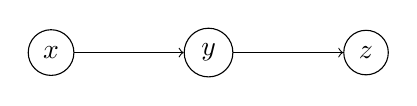
\begin{tikzpicture}
            \node[draw, circle] (x) at (0,0) {$x$};
            \node[draw, circle] (y) at (2,0) {$y$};
            \node[draw, circle] (z) at (4,0) {$z$};
            \draw[->] (x) -- (y);
            \draw[->] (y) -- (z);
        \end{tikzpicture}
    \end{center}
    \item Common cause $x \perp z | y$
    \begin{center}
        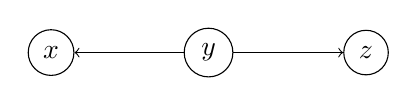
\begin{tikzpicture}
            \node[draw, circle] (x) at (0,0) {$x$};
            \node[draw, circle] (y) at (2,0) {$y$};
            \node[draw, circle] (z) at (4,0) {$z$};
            \draw[->] (y) -- (x);
            \draw[->] (y) -- (z);
        \end{tikzpicture}
    \end{center}
    \item v-structure $x \perp z$ but $x \not\perp z | y$
    \begin{center}
        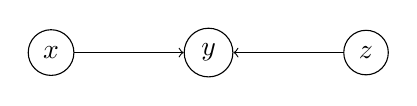
\begin{tikzpicture}
            \node[draw, circle] (x) at (0,0) {$x$};
            \node[draw, circle] (y) at (2,0) {$y$};
            \node[draw, circle] (z) at (4,0) {$z$};
            \draw[->] (x) -- (y);
            \draw[->] (z) -- (y);
        \end{tikzpicture}
    \end{center}
    \end{itemize}
}

  \subsection*{Training}
  \wde{Loss Function}{
    Given a predicted output $\hat y$ and observed output $y$,
    the loss function measures how close the model's prediction is
}
\wde{Zero-One Loss}{
    $L(y, \hat y) = \mathbb{I}_{ \{ y \neq \hat y \} }$ 
}
\wde{Mean Squared Error (MSE)}{
    $L(y, \hat y) = (y - \hat y)^2$
}
\wde{Hinge Loss}{
    $L(y, \hat y) = \max(0, 1 - y \cdot \hat y)$
}
\wde{Gradient Descent}{
    The gradient descent algorithm is given by
    $$
    x_{t+1} = x_t - \eta \nabla f(x_t)
    $$
    where $\eta$ is the learning rate/step size.
}
% sublinear, linear and quadratic convergence
\wde{Convergence}{
    Given $\epsilon > 0$, we say that an algorithm converges to a point $x^*$ if 
    $$
    f(x_t) - f(x^*) \leq \epsilon 
    $$
}
\wde{Convergence Rate}{
    The convergence rate of an algorithm is the rate at which the algorithm converges to the optimal point.
    There are three types of convergence rates:
    \begin{itemize}
        \item Sublinear: $f(x_t) - f(x^*) \leq \frac{c}{t^2}$ ($\epsilon = O(\frac{1}{t^2})$,$ t = O(\frac{1}{\sqrt{\epsilon}})$)
        \item Linear: $f(x_t) - f(x^*) \leq cr^t$ ($\epsilon = O(r^t)$,$t = O(\log \frac{1}{\epsilon})$)
        \item Quadratic: $f(x_t) - f(x^*) \leq c r^{2^t}$ 
    \end{itemize}
}
\wa{Stochastic Gradient Descent (SGD)}{
    Sample a random point $x_t, y_t$ from the dataset and compute the gradient at that point.
    Repeat until solution is satisfactory.
}
\wa{Mini-batch Gradient Descent}{
    Sample a mini-batch of points $x_t, y_t$ from the dataset and compute the gradient at that point.
    Repeat until solution is satisfactory.
}
\wde{Training}{
    The act of minimising the loss function by adjusting the model's parameters
    is known as training.
}

  \subsection*{Regression}
  \wde{Regression}{
    The learning of relationships between input variables $x$ and a 
    numerical output $y$
}
\wde{Feature Transformation}{
    We call $\phi$ a feature transformation. It transforms the input space $X$ into a new space $Z$.
}
\wde{Linear Regression}{
    Given a dataset $S = \{ (\phi(x_1), y_1), \ldots, (\phi(x_n), y_n) \}$,
    minimise the MSE loss function
    $$
    L = \frac{1}{n} \sum_{i=1}^n (y_i - \hat y_i)^2
    $$
    where $\hat y_i = w^T\phi(x_i)$
}
\wde{Closed-form Solution}{
    The closed-form solution to linear regression is given by
    $$
    w = (\Phi\Phi^T)^{-1}\Phi y
    $$
}
\wde{Probalistic Interpretation}{
    The probabilistic interpretation of linear regression is that
    $$
    y = w^T\phi(x) + \epsilon_i
    $$
    where $\epsilon_i \sim \mathcal{N}(0, 1)$ which 
    implies $y_i \sim \mathcal{N}(w^T\phi(x_i), 1)$.
    So the log likelihood (L) of the data is
    $$
    L = \sum_{i=1}^N \left[ -\frac{1}{2} \log(2\pi) - \frac{1}{2} (y_i - w^T\phi(x_i))^2 \right]
    $$
}


  \subsection*{Classification}
  \wde{Classification}{
    Given a dataset $S$, the goal is to learn a function $h$ that maps 
    input variables $x$ to $y$, where $y$ is a class label. 
}
\wde{Linear Seperability}{
    A dataset is linearly seperable if there exists a hyperplane that can seperate the data points
}
\wde{Training of Classification}{
    Find parameters $\theta$ such that the zero-one loss is minimised
}
\wde{Logistic Regression}{
    A linear classifier that models the probability of a class label.
    The model is given by
    $$
    p(y|x, \theta) = \sigma(-y\theta^Tx) = \frac{1}{1 + \exp(-y (\dotp{w}{x} + b))}
    $$
    where $\sigma$ is the sigmoid function.
}
\wde{Maximum Likelihood Estimation (MLE)}{
    The MLE of the parameters $\theta$ is given by
    $$
    \hat \theta = \argmax_\theta \prod_{i=1}^n p(y_i|x_i, \theta)
    $$
}
\wde{Log Likelihood}{
    The log likelihood is applying log to the MLE
    to obtain a more numerically stable solution:
    $$
    L = \sum_{i=1}^n \log p(y_i|x_i, \theta)
    $$
}   
\wa{Training of Logistic Regression}{
    The training of logistic regression is done by maximising the log likelihood $L$ of $w$ and $b$.
    $$
    L = \sum_{i=1}^n \log p(y_i|x_i, \theta)
    $$
    There are no closed-form solutions to this problem, so iterative methods like gradient ascent are used
    which is equivalent to minimising the negative log likelihood. 
}
\wde{Multiclass Classification}{
    Using the softmax function, we can extend logistic regression to multiclass classification.
    Softmax is defined as
    $$
    \operatorname{softmax}\left( \begin{bmatrix} z_1 \\ z_2 \\ \vdots \\ z_k \end{bmatrix} \right) = \begin{bmatrix} \frac{e^{z_1}}{\sum_{i=1}^k e^{z_i}} \\ \frac{e^{z_2}}{\sum_{i=1}^k e^{z_i}} \\ \vdots \\ \frac{e^{z_k}}{\sum_{i=1}^k e^{z_i}} \end{bmatrix}
    $$
}
\wde{Support Vector Machine (SVM)}{
    A linear classifier that finds the hyperplane that maximises the margin between the classes. It 
    does so by solving the following optimisation problem:
    $$
    \min_{w} \frac{1}{2} \norm{w}^2 \quad \text{s.t.} \quad y_i(w^Tx_i + b) \geq 1
    $$
    So the lagrangian is 
    $$
    L(\alpha, w) = \frac{1}{2} \norm{w}^2 - \sum_{i=1}^n \alpha_i(y_i(w^Tx_i + b) - 1)
    $$
}
\wde{Kernel}{
    A kernel $k : \mathbb{R}^d \times \mathbb{R}^d \to \mathbb{R}$ is defined as 
    $$
    k(x, x') = \phi(x)^T\phi(x')
    $$ for some feature function $\phi$.
    It is a measure of similarity between two points in the input space.
}
\we{Common Kernels}{
    \begin{itemize}
        \item Linear: $k(x, x') = x^Tx'$
        \item Polynomial: $k(x, x') = (x^Tx' + 1)^d$
        \item Gaussian: $k(x, x') = \exp\left( -\frac{\norm{x - x'}^2}{2\sigma^2} \right)$
        \item Hyperbolic Tangent: $k(x, x') = \tanh(kx^Tx' + c)$    
    \end{itemize}
}
\wde{Making Kernels}{
    A kernel should satisfy 
    \begin{itemize}
        \item $k(x,z) = \inner{\phi(x)}{\phi(z)} = \inner{\phi(z)}{\phi(x)} = k(z,x)$ (symmetric)
        \item $k(z,x)^2 = k(x,x)k(z,z)$
        \item 
        \begin{align*}
        K = 
        \begin{bmatrix} k(x_1, x_1) & \cdots & k(x_1, x_n) \\ \vdots & \ddots & \vdots \\ k(x_n, x_1) & \cdots & k(x_n, x_n) \end{bmatrix}
        \end{align*}
        is positive semi-definite
    \end{itemize}
}

\wt{Mercer's Theorem}{
    Supoose $k$ is a continuous symmetric non-negative definite kernel, then $k$ can be expressed as 
    $$
    k(x,z) = \sum_{i=1}^\infty \lambda_i \phi_i(x)\phi_i(z)
    $$
    where $\{\phi \}$ are eigen-functions, $\norm{\phi_i} = 1$ and $\{\lambda_i\}$ are positive eigen values $\lambda_i \geq 0$.    
}

\wde{Kernel Trick}{
    The kernel trick is a method to transform the input space into a higher dimensional space
    without explicitly computing the transformation. This is done by using a kernel function
    $$
    k(x, x') = \phi(x)^T\phi(x')
    $$
    where $\phi$ is the transformation function.
}


  \subsection*{Neural Networks}
  \wde{Perceptron (Single-layer Neural Network)}{
    A simple linear classifier that learns a weight vector $w$ to classify data points.
    The perceptron training algorithm can be used to learn the weights.
    Can model logical functions like AND, OR and NOT.
}
\wt{Universal Approximation Theorem}{
    A single-output node NN with  a single hidden layer with 
    finite neurons can app    finite neurons can approximate continuous (and discontinuous) functions
} 
\wde{Multi-layer Perceptron (MLP) / Feedforward Neural Netword (FNN)}{
    A neural network with multiple layers of perceptrons.
    The network is feedforward as there are no cycles in the network. 
    It can model complex decision boundaries (piecewise linear) [XOR, etc]
    The perceptron training algorithm can not be used to learn the weights.
}
\wde{Activation Function}{
    Allows for non-linear decision boundaries. They should 
    be differentiable. Also controls the output range to 
    a specific range. Common activation functions are:
    \begin{itemize}
        \item Sigmoid: $\sigma(x) = \frac{1}{1 + e^{-x}}$
        \item Hyperbolic Tangent (tanh): $\tanh(x) = \frac{1-\exp(-2x)}{1+\exp(-2x)}$
        \item ReLU: $f(x) = \max(0, x)$ (faster than tanh)
        \item Leaky ReLu solves the 'dying ReLU' problem
    \end{itemize}
}
\wde{Computation Graph}{
    Represents computation as a directed graph comprising of simple operations 
    on vectors and matrices which allows for automatic differentiation.
}
  

  \subsection{Generalisation}
  \wde{Independtly and Identically Distributed (i.i.d.)}{
    A dataset is said to be i.i.d. if the data points come from the same distribution and are statistically independent of each other.
}
\wde{Training Error}{
    For a training set $S$, the training error for a loss $\ell$ and a program $h$ is defined as 
    $$
        L_S(h) = \frac{1}{n}\sum_{i=1}^{n} \ell(y_i, h(x_i))
    $$
}
\wde{Generalisation Error}{
    For a program $h$, the generalisation error is defined as
    $$
        \L_{\mathcal{D}}(h) = \E_{(x, y) \sim \mathcal{D}}\left[ \ell(y, h(x)) \right]
    $$
    The goal of learning is to minimise the generalisation error.
}
\wde{Hypothesis Class}{
    A hypothesis class $\mathcal{H}$ is a set of possible programs of a particular form.
}
\we{Hypothesis Class Example}{
    The set of all linear functions is a hypothesis class i.e.
    $$
    \mathcal{H}_{lin} = \{ h(x) = w^Tx \mid w \in \mathbb{R}^d \}
    $$
}
\wde{Learning Algorithm}{
    A learning algorithm is a function that takes a data set of size $m$ and returns a function from the 
    hypothesis class $\mathcal{H}$ 
}
\wt{Probably Approximately Correct (PAC)} {
    A hypothesis class $\mathcal{H}$ is PAC-learnable with a learning algorithm $A$ if for any 
    distribution $\mathcal{D}$, and any $\epsilon > 0$ and $0 \leq \delta \leq 1$, there exists 
    $N > 0$ such that for any $n \geq N$:
    $$
    \mathbb{P}_{S \sim \mathcal{D}^n} \left[ L_{\mathcal D }(A(S)) - \min_{h' \in \mathcal{H}} L_{\mathcal{D}}(h') > \epsilon \right] < \delta 
    $$ 
    In other words, with high probability, the program learned by $A$ achieves a similar error to the best program in $\mathcal{H}$.
}
\wde{Empirical Risk Minimisation (ERM)}{
    Minimising the loss on a training set is also known as empirical risk minimisation 
    $$
        A_{ERM, \mathcal{H}(s)} = h_{ERM} = \argmin_{h \in \mathcal{H}} L_S(h)
    $$
}
\wt{No free lunch theorem}{
    Suppose $|\mathcal{X}| = 2m$. For any learning algorithm $A$, there is a distribution $\mathcal{D}$ and 
    $f : \mathcal{X} \to \{0,1\}$ such that $L_\mathcal{D}(f) = 0$, but 
    $$
        \mathbb{P}_{S \sim \mathcal{D}^m} \left[ L_{\mathcal{D}}(A(S)) \geq \frac{1}{10} \right] \geq \frac{1}{10}
    $$
}
\wt{Error Decomposition}{
    $$
    \L_{\mathcal{D}}(h) = \underbrace{L_{\mathcal{D}}(h) - \min_{h' \in \mathcal{H}} L_{\mathcal{D}}(h')}_{\text{Estimation Error}} + \underbrace{\min_{h' \in \mathcal{H}} L_{\mathcal{D}}(h') - L_S(h)}_{\text{Approximation Error}} 
    $$
}
\wde{Uniform Convergence}{
    A hypothesis class $\mathcal{H}$ has uniform convergence property if for any distribution 
    $\mathcal{D}$, and any $\epsilon > 0$ and $0 \leq \delta \leq 1$, there exists $N > 0$ such that for any $n \geq N$ and every $h \in \mathcal{H}$:
    $$
    \mathbb{P}_{S \sim \mathcal{D}^n} \left[ |L_{S}(h) - L_{\mathcal{D}}(h)| > \epsilon \right] < \delta
    $$
}
\wt{Uniform Convergence implies PAC learnability}{
    If a hypothesis class $\mathcal{H}$ has the uniform convergence property, then it is PAC learnable with ERM.
}
\wde{Shattering}{
    A set of $n$ points is shattered by $\mathcal{H}$ if there is an arrangement of $n$ points such 
    that classifiers in $\mathcal{H}$ can produce all $2^n$ ways of labelling the points.
}
\wde{Vapnik-Chervonenkis (VC) Dimension}{
    VC Dimension is the largest number of points that $\mathcal{H}$ can shatter
}

\wde{VC Generalisation Bounds}{
    With probability $1 - \delta$, for all $h \in \mathcal{H}$:
    $$
    L_{\mathcal{D}}(h) \leq L_S(h) + 2 \sqrt{\frac{8d \log (en/d) + 2 \log(4/\delta)}{n}}
    $$
    d is the VC dimension of $\mathcal{H}$.
}
\we(VC Dimension){
    \begin{itemize}
        \item For linear classifers, $\VC(\mathcal{H}_{lin}) = p + 1$
        % \item For polynomial classifiers of degree $p$, $\VC(\mathcal{H}_{poly}) = \binom{p+d}{d}$
        \item For MLP with $p$ edges, $\VC(\mathcal{H}_{mlp}) = O(p\log p)$
    \end{itemize}
}
\wde{Surrogate Loss}{
    A surrogate loss is a loss function that is easier to optimise than the original loss function.
    Cross entropy or log likelihood are common surrogate losses for 0-1 loss.
}
\wde{Underfitting}{
    A model $h$ is underfitting if there is another model $f$ that has a lower training i.e. 
    $L_S(f) < L_S(h)$.
}
\wde{Overfitting}{
    A model $h$ is overfitting if there is another model $f$ that has a higher training error ($S$)
    but a lower test error ($S'$) i.e. $L_{S}(f) > L_S(h)$ and $L_{S'}(f) < L_{S'}(h)$.
}
\wde{Development Set}{
    A development set is a subset of the training set that is used to tune hyperparameters.
}
\wde{Stability}{
    A learning algorithm is stable if the learned program does not change much in
    performance when we change the data set slightly. 
}
\wt{Stability prevents Overfitting}{
    Stable learning algorithms don't overfit
}
\wde{$\lambda$-strongly convex}{
    A function $f$ is $\lambda$-strongly convex if for all $x, y$ and $\lambda > 0$:
    $$
    f(y) \geq f(x) + \dotp{\nabla f(x)}{y - x} + \frac{\lambda}{2}\norm{y - x}^2
    $$
}
\wt{$L_2$ Regularisation}{
    Regularisation is a technique to prevent overfitting by adding a penalty term to the loss function.
    For $L_2$ regularisation, the loss function is modified to
    $$
    L = \frac{1}{n} \sum_{i=1}^n \ell(y_i, h(x_i)) + \frac{\lambda}{2}\norm{w}^2
    $$
    Note that if the loss function is convex, then the regularised loss function is $\lambda$-strongly convex.
}
\wde{Hardness of Optimising Neural Networks}{
    Training a 2-layer 3 node neural network is NP-complete.
    If we could minimise the loss function in polynomial time, then we would 
    be able to solve the P=NP problem.
}
\wde{Overparameterisation}{
    Overparameterisation is the practice of using more parameters than necessary to fit the training data.
    It helps with optimisation.
}
\wde{Interpolation}{
    A model interpolates the data if it achieves zero training error.
}


  \subsection{PCA}
  \wde{Dimensionality Reduction}{
    Dimensionality reduction is the process of reducing the number of features in a dataset.
    This is used for visualisation, exploration and compression.
}
\wde{Principal Component Analysis (PCA)}{
    PCA is a method for dimensionality reduction. It finds the directions that maximise the variance in the data. These 
    directions are called principal components. Each principle component is orthogonal to the others. 
}
\wde{Maximum Variance Formulation}{
    An optimisation problem that PCA solves is to find the directions that maximise the variance in the data.
    This can be solved with lagrange multipliers. 
}
  \subsection*{Expectation Maximisation}
  \wde{
    Expectation Maximisation 
}{
    If can't solve an optimisation problem directly, EM is used. It yields a lower bound of the original loss. It utilises Jensen's inequality.
}

\wde{K-means Distortion}{
    $$
    J = \sum^N_{n = 1}\sum^K_{k = 1} r_{nk} \Vert x_n - \mu_k \Vert^2
    $$
}
\wde{K-means Steps}{
 \begin{itemize}
 \item Randomly initialise $\mu_{k = 1,\dots, K}$ 
 \item Minimise $J$ with respect to $r_{nk}$ (Expectation)
 \item Minimise $J$ with respect to $\mu_{k}$ (Maximisation) 
 \item Repeat until convergence
 \end{itemize}
}
\wde{K-means Solutions}{
    $$\mu_k = \frac{\sum_n r_{nk} x_n}
    % {\sum_n r_{nk}}, r_{nk} = \mathbb{I}
    {\underbrace{\sum_n r_{nk}}_{\text{Mean of cluster }}}, 
    (k = \arg\min_j \Vert x_n - \mu_j \Vert ^2)$$
}
\wde{GMM Probabilities}{
    $$p(z_k = 1) = \pi_k, p(\mathbf{z}) = \prod_{k = 1}^K \pi_k^{z_k}, p(\mathbf{x} \vert \mathbf{z}) = \prod_{k = 1}^K \mathcal{N}(x | \mu_k, \Sigma_k)^{z_k}$$
}
\wde{GMM Responsibility Function}{
    $$r_{nk} = p(z_k = 1 \vert x_n) = \frac{\pi_k \mathcal{N}(x_n | \mu_k, \Sigma_k)}{\sum_{j = 1}^K \pi_j \mathcal{N}(x_n | \mu_j, \Sigma_j)}$$
}
\wde{Kullback-Leibler Divergence}{
    Measure how well one probability distribution approximates another 
    $$KL(p\Vert q) = \mathbb{E}_{x \sim p}\left[\log \frac{p(x)}{q(x)}\right] = \sum_{x \in X} p(x) \log \frac{p(x)}{q(x)}$$ 
    Not a metric as it is not symmetric $KL(p\Vert q) \neq KL(q\Vert p)$
}

  %
  % \end{multicols}
  % % \begin{multicols}{2}
  %   \subsection*{Examples}
  % \input{src/examples/l1}
  % \input{src/examples/l2}
  \end{multicols}
\end{document}
